Finalmente hemos implementado una tercera estrategia basada en un algoritmo genético. Dadas las dimensiones del problema (NP-completo), es natural buscar una solución lo suficientemente buena aunque no tenga por qué ser la mejor. Este es exactamente el punto de vista que hemos tomado para abordar esta tercera solución.

Los algoritmos genéticos son un tipo de estrategias clasificadas como metaheurísticas. Esto es, utilizadas en ámbitos muy diversos ya que operan de forma abstracta e independiente al problema en si. En particular, los algoritmos genéticos se basan en la teoría evolutiva de Darwin en la que una población, mediante cruces entre sus individuos y mutaciones, es cada vez más fuerte conformen pasan las generaciones. Para más información sobre el tema:

https://es.wikipedia.org/wiki/Metaheuristica
http://sci2s.ugr.es/graduateCourses/Metaheuristicas
https://es.wikipedia.org/wiki/Algoritmo_geneticos

En un algoritmo genético consideramos un conjunto o población de soluciones (también llamados genes o individuos de la población), inicializadas aleatoriamente, y realizamos distintas operaciones sobre ellas para ir mejorándolas y así obtener soluciones cada vez mejores. En nuestro caso, cada individuo será una permutación de números: el orden en el que recorremos las ciudades.

Las operaciones que se realizan sobre los individuos son operadores de cruce y operadores de mutación:
\begin{itemize}
	\item Los operadores de cruce obtienen uno o varios individuos (hijos) a partir un par de soluciones de la poblacion (padres). En nuestro caso utilizaremos el operador de cruce de orden:
	
	\begin{figure}[H]
		\centering
		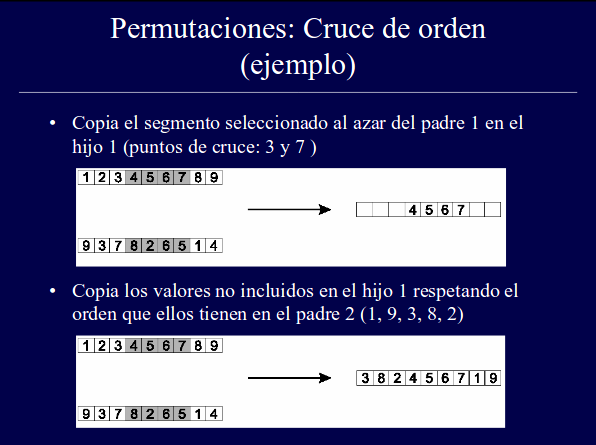
\includegraphics[width=0.8\textwidth]{imag1.jpg}
		\caption{Operador de cruce de orden.}
	\end{figure}
	
	\item Los operadores de mutación están limitados por una cierta probabilidad fijada. Es decir, no todos los individuos de una población mutan. Se aplican sobre un único individuo y lo alteran unicamente a él. En nuestro caso utilizaremos el operador de mutación por inserción:
	
	\begin{figure}[H]
		\centering
		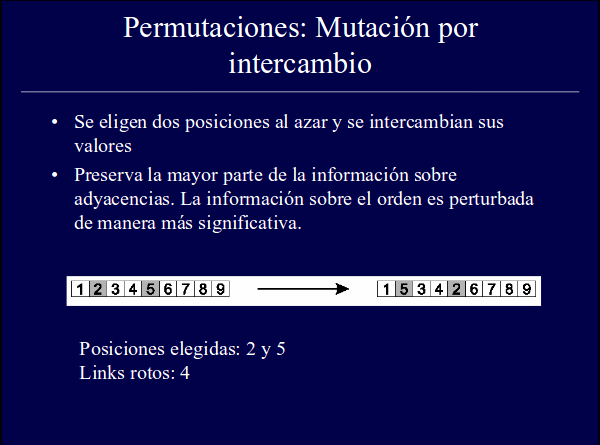
\includegraphics[width=0.8\textwidth]{imag2.jpg}
		\caption{Operador de mutación por intercambio.}
	\end{figure}
	
\end{itemize}
 
Ambos imágenes provienendel siguiente enlace, diapositivas 20 y 17 respectivamente:
http://users.exa.unicen.edu.ar/~icompevol/filminasenpdf/terceraclase.pdf

Además, hemos de medir cuan buena es cada una de nuestras soluciones, necesitamos una \textbf{función de evaluación}. Esta será la longitud de la ruta determinada por la permutación.

Finalmente y antes de explicar el flujo del algoritmo en si hace falta definir un último operador: el de selección. Este operador define como se realiza la selección de padres de una generación (si cogiesemos unicamente los mejores convergeriamos muy rápido a un óptimo local pues no hay diversidad en nuestra población mientras que si se selecciona de forma puramente aleatoria nos estaríamos teniendo en cuenta cuan buena es cada solución). Aplicaremos \textbf{selección por torneo}. En esta estrategia se seleccionan de forma aleatoria un número pequeño de individuos (3 o 5 son valores comunmente utilizados), y de entre estos se escoge el mejor.

Una vez definidos los operadores, el algoritmo en si es sencillo. Realizaremos $n_generaciones$ generaciones a partir de una poblacion de $N$ individuos obtenida aleatoriamente. En cada generación se escogen padres (con el operador de selección) y se cruzan (con el operador de cruce) hasta obtener una nueva generación de $N$ elementos. Estos nuevos individuos se mutan (bajo una probabilidad $mutate_probability$) y finalmente se sustituye la población anterior por la nueva.

\begin{verbatim}
// Initialize the population and evaluate it
InitializePopulation(population, pob_size, n_cities);
best_gen_ever = *population[0];
EvaluatePopulation(population, best_gen_ever, cities);

for (int i=0; i<n_generations; i++) {
	// Obtain the next generation and apply crossover from the elements of population
	ApplySelectionAndCrossover(population, new_generation);
	
	// Apply mutation to the new population with a probability prob
	ApplyMutation(new_generation, mutate_propability);
	
	// Evaluate the new population and save the best solution found
	EvaluatePopulation(new_generation, best_gen_ever, cities);
	
	// Replace the old population with the new one
	ReplaceGeneration(population, new_generation);
}
\end{verbatim}

Nuestra mejor solución está almacenada en $best_gen_ever$.